\documentclass[11pt,a4paper]{article}
\usepackage[margin=2.3cm]{geometry}
\usepackage{tikz}\usetikzlibrary{positioning,arrows.meta}
\usepackage{graphicx,booktabs,amsmath,caption,subcaption,hyperref,float}
\graphicspath{{../plots/}}
\title{Predicting Gata4 HT-SELEX affinities from MD-derived DNA shape:\\ preprocessing and model comparison with new tetramer/hexamer shape tables}
\author{Pieter Zanders}
\date{22 October 2026}
\begin{document}\sloppy
\maketitle
\begin{abstract}
We characterise newly generated tetramer and hexamer DNA-shape tables (average helical parameters and stiffness matrices) and use them to predict Gata4 HT-SELEX 10-mer affinities. All labels come from the SELEX affinity table (\texttt{4.txt}), in which affinity is exactly $0.172\,(\mathrm{obs}/\mathrm{exp})^{1/4}$, only 12.1\% of 10-mers are present and 52.5\% of entries have a single count. We ran a preprocessing ablation under a leakage-free validation scheme (5-fold cross-validation grouping each $k$-mer with its reverse complement, plus a fixed 10\% held-out test set). Four choices worked best: log-affinity labels, a count threshold of $\geq$10, per-strand labels (no averaging of the two orientations) and tetramer shape features plus per-window one-hot encoding with standardisation. Per-strand labels were much better than merged labels, gaining 0.15--0.17 in CV $R^2$. Hexamer features did not help. Under the same protocol we compared nine regressors and two neural-network ensembles. CNN1D was the best single model (held-out test $R^2=0.736\pm0.012$, Pearson 0.860, Spearman 0.844; 0.788 for the averaged prediction of its 15 runs). It was followed by CNNAttention (0.725), the Transformer (0.685), DFN and LightGBM (both 0.644), SVR (0.598), random forest (0.572) and linear/ridge regression (0.47). An ensemble of CNN1D and CNNAttention reached 0.785 and an ensemble of all four NNs 0.756. The shape features improved tree models but added nothing to the CNN beyond one-hot encoding. The supplied \texttt{SELEX\_test.txt} is not consistent with \texttt{4.txt} and was not used for evaluation.
\end{abstract}

\section{Introduction}
Transcription factors (TFs) recognise their genomic targets through direct base readout and through the sequence-dependent three-dimensional shape of DNA (``shape readout'') \cite{rohs2009}. High-throughput SELEX (HT-SELEX) enriches DNA ligands bound by a TF over successive selection rounds and sequences them, giving large-scale relative affinities for $k$-mers \cite{jolma2013}. Physics-based descriptors from atomistic molecular dynamics (MD) summarise the local structure and flexibility of DNA. Examples are average base-step helical parameters (shift, slide, rise, tilt, roll, twist) and stiffness (force-constant) matrices. Such descriptors can complement or replace the raw sequence as model input, and they give an interpretable view of affinity determinants. DNAffinity builds regressors on such features. Here we test new tetramer- and hexamer-level shape tables on Gata4 HT-SELEX data and ask (i) which preprocessing is optimal and (ii) how classical and deep models compare.

\section{Methods}
\subsection{Affinity labels}
Labels are taken from the SELEX package output for Gata4 (\texttt{data/selex/Gata4/4.txt}). It has 126{,}624 10-mers with observed and expected (Markov-model) counts, affinity and SE. We verified that $\mathrm{Affinity}=0.172\,(\mathrm{obs}/\mathrm{exp})^{0.25}$ to machine precision (sd of the ratio $2.5\times10^{-16}$) and that $\mathrm{SE}\sqrt{n}/\mathrm{Aff}$ has median $1.414\approx\sqrt2$. The table is zero-truncated: only 12.1\% of the $4^{10}$ possible 10-mers appear. 52.5\% of entries have count 1, and 13{,}100 have count $\geq$10. Because the SE is about $\sqrt2\,\mathrm{Aff}/\sqrt n$, labels with low counts are very noisy.

\subsection{Shape features}
The new tables \texttt{data/selex/tetramer/\{avg,fce\}\_tetramer.dat} and \texttt{data/selex/hexamer/\{avg,fce\}\_hexamer.dat} give, for every tetramer (256) and hexamer (4096), six average helical parameters (\texttt{avg}) and a flattened $6\times6$ stiffness matrix (\texttt{fce}). The matrices are exactly symmetric and positive definite (minimum eigenvalue $\approx 0.006$), so we keep the 21 unique upper-triangle entries. A 10-mer is represented by 7 overlapping tetramer windows (and 5 hexamer windows). Hexamer $j$ is aligned to its central tetramer window $j{+}1$ and zero-padded at the ends for windowed models. Optional one-hot input adds the 16 one-hot values of the bases in each tetramer window. Flat models use the concatenated windows; windowed models (CNN1D, CNNAttention, Transformer) use a $7\times d$ tensor.

\subsection{Data processing pipeline}\label{sec:pipeline}
All steps are implemented in \texttt{scripts/selex\_new\_shape/lib.py} (functions \texttt{load\_labels}, \texttt{split}, \texttt{flat\_feats}, \texttt{windowed}, \texttt{tf}) and \texttt{train\_final.py}. Figure~\ref{fig:pipe} summarises them.

\begin{figure}[H]\centering
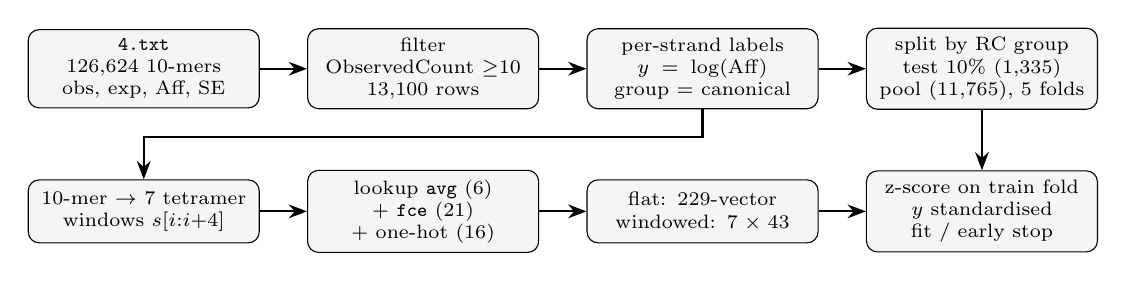
\begin{tikzpicture}[node distance=4mm and 6mm, every node/.style={font=\scriptsize}, box/.style={draw, rounded corners, align=center, minimum height=8mm, text width=27mm, fill=gray!8}, arr/.style={-Stealth, thick}]
\node[box] (a) {\texttt{4.txt}\\126{,}624 10-mers\\obs, exp, Aff, SE};
\node[box, right=of a] (b) {filter\\ObservedCount $\geq$10\\13{,}100 rows};
\node[box, right=of b] (c) {per-strand labels\\$y=\log(\mathrm{Aff})$\\group = canonical};
\node[box, right=of c] (d) {split by RC group\\test 10\% (1{,}335)\\pool (11{,}765), 5 folds};
\node[box, below=9mm of a] (e) {10-mer $\to$ 7 tetramer\\windows $s[i{:}i{+}4]$};
\node[box, right=of e] (f) {lookup \texttt{avg} (6)\\+ \texttt{fce} (21)\\+ one-hot (16)};
\node[box, right=of f] (g) {flat: 229-vector\\windowed: $7\times43$};
\node[box, right=of g] (h) {z-score on train fold\\$y$ standardised\\fit / early stop};
\draw[arr] (a)--(b); \draw[arr] (b)--(c); \draw[arr] (c)--(d);
\draw[arr] (e)--(f); \draw[arr] (f)--(g); \draw[arr] (g)--(h); \draw[arr] (d)--(h);
\draw[arr] (c.south) |- ++(0,-3.5mm) -| (e.north);
\end{tikzpicture}
\caption{Processing pipeline for the chosen configuration. Row counts are those of the final runs.}\label{fig:pipe}\end{figure}

\subsubsection{Reading and checking the labels}
\texttt{4.txt} (tab-separated, quoted header, R row names) is read with pandas. The columns used are \texttt{Kmer}, \texttt{ObservedCount} ($n$), \texttt{ExpectedCount} ($e$, from the Markov background model of round 0) and \texttt{Affinity}. We checked that
\begin{equation}
\mathrm{Aff} = 0.172\,(n/e)^{1/4}, \qquad \mathrm{SE}\approx \sqrt{2}\,\mathrm{Aff}/\sqrt{n},
\end{equation}
so $\mathrm{SE}/\mathrm{Aff}=\sqrt{2/n}$: 141\% at $n=1$ and 45\% at $n=10$. The table is zero-truncated. Only $k$-mers seen at least once in the selected round are listed (12.1\% of $4^{10}$), and there are no entries for unobserved, low-affinity $k$-mers. The models therefore learn on the observed range only.

\subsubsection{Count filter}
Rows with $n\geq10$ are kept (\texttt{load\_labels(min\_count=10)}), leaving 13{,}100 of 126{,}624 rows. This bounds the relative SE at about 45\%. The ablation (Table~\ref{tab:abl}) chose this threshold.

\subsubsection{Per-strand vs.\ merged labels}
Each row's group key is the canonical sequence $\min(s,\mathrm{rc}(s))$, with \texttt{canonical} from \texttt{dnaffinity.preprocess}.
\begin{itemize}
\item \emph{Per-strand} mode (chosen) keeps each measured orientation as its own row with its own label. A reverse-complement row exists only if that orientation itself passed the filter. The 13{,}100 rows form 10{,}771 groups.
\item \emph{Merged} mode averages the affinities of the measured orientations per group and emits the canonical sequence and its reverse complement with the same label (reverse-complement augmentation).
\end{itemize}

\subsubsection{Label transform}
The target is $y=\log(\mathrm{Aff})=\tfrac14\log(n/e)+\log 0.172$, i.e.\ a scaled log-enrichment. Inside each training fold, $y$ is also standardised for model fitting, $\tilde y=(y-\bar y_\mathrm{tr})/s_\mathrm{tr}$, and predictions are transformed back. All metrics are computed on $y$.

\subsubsection{Windowing and shape lookup}
A 10-mer $s$ is cut into the $7$ overlapping tetramers $s[i{:}i{+}4]$, $i=0,\dots,6$ (each describes the central base step of its window). For each window we look up:
\begin{itemize}
\item the 6 averages of \texttt{avg\_tetramer.dat} (shift, slide, rise, tilt, roll, twist);
\item the 21 upper-triangle entries (including the diagonal) of the symmetric $6\times6$ stiffness matrix in \texttt{fce\_tetramer.dat}. The 36 stored values contain 15 duplicates.
\end{itemize}
Hexamer tables, used only in the ablation, are read the same way. A flat vector concatenates the 5 hexamers $s[j{:}j{+}6]$. In windowed form, hexamer $j$ is placed at tetramer position $j{+}1$, i.e.\ aligned on its central tetramer, and the two end positions are zero-padded.

\subsubsection{One-hot encoding}
\emph{What it does.} One-hot encoding turns each base into a 4-dimensional binary vector with a single 1 at the position of that base in the fixed order (A, C, G, T): $\mathrm{A}\to(1,0,0,0)$, $\mathrm{C}\to(0,1,0,0)$, $\mathrm{G}\to(0,0,1,0)$, $\mathrm{T}\to(0,0,0,1)$ (\texttt{lib.OH}).

\emph{Why it is needed.} The shape tables describe each tetramer only indirectly, through 27 physical numbers. One-hot gives the models the sequence identity itself. Coding bases as integers (e.g.\ A=0, \dots, T=3) would impose a false order and spacing (T ``larger'' than A, G ``between'' C and T). One-hot has no such ordinal bias: all four bases are equidistant, and every weight that multiplies a channel is specific to one base at one position, like a position weight matrix.

\emph{Layout in \texttt{lib.py}.}
\begin{itemize}
\item \textbf{Flat models} (\texttt{flat\_feats}): the 10 bases of the 10-mer are encoded in order and concatenated, giving $10\times4=40$ values. They come after the shape block: $[\texttt{avg}\,(42),\ \texttt{fce}\,(147),\ \text{one-hot}\,(40)]$ for set (a). Channel $4j+n$ of the one-hot block is 1 if base $j$ ($j=0..9$) is nucleotide $n$.
\item \textbf{Windowed models} (\texttt{windowed}): at tetramer window $i$ ($i=0..6$, bases $s[i{:}i{+}4]$) the 4 bases of the window are encoded and concatenated, giving 16 values per position. They are appended after the 27 shape channels of the same window, so each position has $[\texttt{avg}\,(6),\ \texttt{fce}\,(21),\ \text{one-hot}\,(16)] = 43$ channels. Because consecutive windows overlap by 3 bases, every internal base appears in up to 4 windows, at a different offset in each.
\item \textbf{One-hot only} (set (d), \texttt{shape=0}): the shape block is omitted, giving 40 flat values or $7\times16$.
\end{itemize}

\emph{Worked example.} For the tetramer window GATA:
\[
\mathrm{G}\,(0,0,1,0)\ \|\ \mathrm{A}\,(1,0,0,0)\ \|\ \mathrm{T}\,(0,0,0,1)\ \|\ \mathrm{A}\,(1,0,0,0)\ =\ (0,0,1,0,\ 1,0,0,0,\ 0,0,0,1,\ 1,0,0,0).
\]
In a windowed model these 16 values are concatenated with the 6 \texttt{avg} values (SHIFT, SLIDE, RISE, TILT, ROLL, TWIST) and the 21 \texttt{fce} values that the shape tables give for GATA.

\emph{Combination with shape.} Shape and one-hot are concatenated, never multiplied. Like all features, the one-hot channels are then z-scored with the training-fold mean and sd. A channel $x\in\{0,1\}$ with frequency $p$ becomes $(x-p)/\sqrt{p(1-p)}$, so an absent base gets a non-zero (negative) value. The shape features are a deterministic function of the tetramer and hence of its 16 one-hot values. A model can therefore read sequence identity directly (one-hot) and/or use the physical summary (shape). This redundancy is what the one-hot-only benchmark (d) and the LRP analysis test.

\subsubsection{Feature tensors per model}
\begin{itemize}
\item \textbf{Flat} (Linear, Ridge, SVR, RF, DFN): $[\texttt{avg}_{0..6}\,(42),\ \texttt{fce}_{0..6}\,(147),\ \text{one-hot}\,(40)]$, i.e.\ a 229-dimensional vector (\texttt{flat\_feats}).
\item \textbf{Windowed} (CNN1D, CNNAttention, Transformer): a $7\times43$ tensor whose channels per position are $[\texttt{avg}\,(6),\texttt{fce}\,(21),\text{one-hot}\,(16)]$ (\texttt{windowed}).
\end{itemize}

\subsubsection{Standardisation}
Within each CV fold, features are z-scored with means and standard deviations computed on the training-fold rows only and applied to all rows (validation and test). For windowed input the statistics are pooled over samples and positions per channel. Because of this external scaling, the input \texttt{LayerNorm} of the PyTorch models was switched off (\texttt{normalization=False}).

\subsubsection{Splits}
\texttt{split()} draws 10\% of all canonical groups in \texttt{4.txt} (seed 20) as the test set. This gives 1{,}335 test rows and 11{,}765 pool rows after filtering, the same set for every model and configuration. The pool is partitioned by \texttt{GroupKFold(5)} on the canonical group, so a $k$-mer and its reverse complement are always on the same side. For NNs, a further random 10\% of each training fold (seed $100+k$ for fold $k$) is the early-stopping set, and reported ``train'' metrics include it.


\subsection{Validation protocol}
Every $k$-mer is grouped with its reverse complement. A fixed random 10\% of groups (seed 20, drawn over all groups in \texttt{4.txt}) forms the held-out test set. The remaining pool is split by \texttt{GroupKFold} into 5 folds. Inside each training fold, neural networks and LightGBM hold out a random 10\% for early stopping. For every fold model we report train-fold, validation-fold and test metrics. Metrics are $R^2$, Pearson and Spearman correlations on log affinity, given as mean$\pm$sd over folds (and seeds), plus the train--test $R^2$ gap. The ``averaged-runs'' test $R^2$ is the $R^2$ of the mean prediction of all fold/seed models of one type.

\subsection{Preprocessing ablation}
Starting from a base configuration (log label, count $\geq$10, per-strand labels, tetramer avg+fce, standardisation), we changed one factor at a time and scored a random forest (300 trees, min leaf 3, max features 0.33) and a CNN1D (one seed). The factors were: label transform (raw vs log), count threshold (1, 3, 10, 30), merged vs per-strand labels, feature tables (tetramer, hexamer, both), \texttt{avg}/\texttt{fce}/both, one-hot $\pm$ shape, and standardisation. Merged labels average the measured strands per canonical $k$-mer and emit both orientations (reverse-complement augmentation). Per-strand labels keep each measured orientation as its own row. To make configurations comparable, every one was scored on the same rows: held-out-fold rows with a measured per-strand label and count $\geq$10. The CNN was not run at thresholds 1 and 3 because of CPU cost.

\subsection{Models}\label{sec:models}
The repository models are used through their \texttt{dnaffinity.models} classes. The architectures below are taken from that code (repository \texttt{PieterZanders/DNAffinity}, branch \texttt{deep-learning}). Parameter counts are for our $229$-feature / $7\times43$ inputs.

\paragraph{Shared PyTorch training loop} (\texttt{torch\_base.TorchRegressor}).
\begin{itemize}
\item AdamW optimiser, MSE loss (Huber optional) and gradient-norm clipping at 5.
\item ReduceLROnPlateau (factor 0.5, patience $\lfloor\text{patience}/3\rfloor$).
\item Early stopping on the validation loss, with the best weights restored.
\item Shuffled mini-batches; batches of size 1 are skipped because of BatchNorm.
\item Our settings: batch size 64, at most 300 epochs, patience 25, weight decay $10^{-2}$, 3 seeds (0, 1, 2) per fold.
\end{itemize}

\subsubsection{Linear regression}
\texttt{dnaffinity.models.Linear} wraps scikit-learn \texttt{LinearRegression} (ordinary least squares, no penalty).
\begin{itemize}
\item \emph{Pros:} convex, deterministic and fast. The coefficients can be read directly.
\item \emph{Cons:} it cannot represent interactions or non-linear dependence on shape.
\item \emph{Biological relevance:} on the one-hot block it is an additive, position-independent model, equivalent to a position weight matrix (PWM) on log affinity. On the shape block it is an additive model of base-step geometry and stiffness.
\item \emph{Observed:} it underfits (train $R^2$ 0.50, test 0.47, gap 0.03). Additivity explains about half of the variance of log affinity.
\end{itemize}

\subsubsection{Ridge regression}
\texttt{dnaffinity.models.Ridge} wraps scikit-learn \texttt{Ridge} (L2 penalty). The repository default is $\alpha=1$; we used $\alpha=10$.
\begin{itemize}
\item \emph{Pros:} the penalty stabilises the strongly collinear shape features (overlapping windows, correlated parameters).
\item \emph{Cons:} same additive limit as linear regression.
\item \emph{Observed:} practically identical to linear regression (test 0.470). With 11.7k rows and 229 features the variance of OLS is already small, so the limitation is bias, not variance.
\end{itemize}

\subsubsection{Support vector regression}
\texttt{dnaffinity.models.SVR} wraps scikit-learn \texttt{SVR} with the repository defaults: RBF kernel, $C=1$, $\varepsilon=0.1$, $\gamma=\text{`scale'}$, on standardised inputs and targets.
\begin{itemize}
\item \emph{Pros:} a smooth non-linear kernel model that captures interactions implicitly and is robust thanks to the $\varepsilon$-insensitive loss.
\item \emph{Cons:} cost grows between quadratically and cubically with the number of samples. It is not interpretable, and the isotropic RBF kernel treats all 229 features alike.
\item \emph{Biological relevance:} similarity in kernel space means sequences with similar shape and base profiles get similar affinity, a nearest-neighbour view of the binding landscape.
\item \emph{Observed:} test 0.598, gap 0.146, better than RF.
\end{itemize}

\subsubsection{Random forest}
\texttt{dnaffinity.models.RandomForest} wraps scikit-learn \texttt{RandomForestRegressor} (repository defaults: 200 trees, \texttt{max\_features}=1.0). We used 500 trees, \texttt{min\_samples\_leaf}=3 and \texttt{max\_features}=0.33.
\begin{itemize}
\item \emph{Pros:} non-parametric and indifferent to feature scale. It gives feature importances that can rank shape parameters per window.
\item \emph{Cons:} axis-aligned splits approximate smooth effects poorly. Deep trees memorise noisy labels.
\item \emph{Biological relevance:} threshold rules on single shape parameters (e.g.\ ``roll at step 4 above $x$'') are directly readable as indirect-readout hypotheses \cite{rohs2009}.
\item \emph{Observed:} largest gap (train 0.884, test 0.572). It is also the model that benefited most from shape on top of one-hot in the ablation (0.563 $\to$ 0.599), because the shape tables give trees ready-made smooth physical covariates.
\end{itemize}

\subsubsection{DFN (deep feedforward network)}
\texttt{dfn.DFN} builds \texttt{FeedForward}: \texttt{nn.Linear} layers with \texttt{ReLU} and \texttt{Dropout} after every hidden layer and no activation on the output. It is wrapped in \texttt{RegressionCV}, which adds an optional input \texttt{LayerNorm} (disabled here). The repository default layers are \texttt{[64,32,1]} (and \texttt{[256,128,64,32,1]} with lr $10^{-4}$ for SELEX in \texttt{common.py}). We used \texttt{[256,128,64,1]} (229$\to$256$\to$128$\to$64$\to$1, 100{,}097 parameters), dropout 0.2 and lr $3\times10^{-4}$.
\begin{itemize}
\item \emph{Pros:} a universal approximator on the flat vector that can learn any interaction.
\item \emph{Cons:} no positional inductive bias (a motif shifted by one window is a new pattern), so it needs more data and overfits easily.
\item \emph{Observed:} test 0.644, gap 0.176, best epoch 44 of 70, the best flat model.
\end{itemize}

\subsubsection{CNN1D}
\texttt{cnn1d.CNN1DRegressor} builds \texttt{CNN1D} (60{,}481 parameters):
\begin{itemize}
\item optional input \texttt{LayerNorm} (off);
\item stem \texttt{Conv1d}(43$\to$64, kernel 3, padding 1) + \texttt{BatchNorm1d} + \texttt{ReLU};
\item 2 \texttt{ResidualConvBlock}s, each Conv1d(64,64,3)--BN--ReLU--Conv1d(64,64,3)--BN, a skip connection, then ReLU;
\item global average pooling over the 7 positions;
\item \texttt{MLPHead}: Linear(64$\to$32)--ReLU--Dropout--Linear(32$\to$1).
\end{itemize}
We used the repository defaults (hidden 64, 2 blocks, kernel 3, average pooling) with dropout 0.2 and lr $10^{-3}$.
\begin{itemize}
\item \emph{Pros:} weight sharing gives translation equivariance, so the same filter detects a feature at every position. Capacity is moderate.
\item \emph{Cons:} the receptive field is limited by depth (here the 2 blocks plus stem cover the whole 7-window input). Pooling discards absolute position.
\item \emph{Biological relevance:} first-layer filters over one-hot channels act like PWMs/motif detectors, and stacked convolutions combine adjacent sub-motifs. Pooling encodes the idea that a site can sit at any offset in the 10-mer, which matters here because the top $k$-mers are shifted overlaps of the same motif.
\item \emph{Observed:} best single model (test 0.736, 0.788 for averaged runs). It overfits after epoch $\approx$27 (final train MSE 0.068 vs.\ best validation 0.261), which early stopping controls. Shape channels were redundant given one-hot: 7 windows with 16 one-hot channels already determine the tetramer, so the network can learn any per-tetramer lookup itself.
\end{itemize}

\subsubsection{CNNAttention}
\texttt{cnn\_attention.CNNAttentionRegressor} uses the same \texttt{ConvBackbone} as CNN1D, followed by \texttt{num\_attn\_layers}=1 \texttt{nn.MultiheadAttention} layer (embedding 64, 4 heads, dropout as configured) with a residual connection and \texttt{LayerNorm}, then global average pooling and the same \texttt{MLPHead} (77{,}249 parameters; repository defaults otherwise).
\begin{itemize}
\item \emph{Pros:} attention can couple distant positions, beyond the convolutional receptive field, and its weights can be inspected.
\item \emph{Cons:} more parameters, and little extra range on a length-7 input.
\item \emph{Biological relevance:} pairwise attention can represent dependencies between non-adjacent positions (dinucleotide/epistatic effects, spacing of half-sites), which a PWM ignores.
\item \emph{Observed:} test 0.725, gap 0.155, slightly below CNN1D. For 10-mers the convolutions already see the whole sequence, so attention adds capacity but no new range.
\end{itemize}

\subsubsection{Transformer}
\texttt{transformer.TransformerRegressor} builds the following (19{,}073 parameters):
\begin{itemize}
\item optional input \texttt{LayerNorm} (off) and a \texttt{Linear} projection 43$\to d_\mathrm{model}$;
\item sinusoidal positional encoding and a learnable CLS token prepended;
\item \texttt{nn.TransformerEncoder} with pre-norm layers (\texttt{norm\_first=True}, GELU activation);
\item pooling over the CLS token or the mean of the position tokens;
\item an \texttt{MLPHead} as above.
\end{itemize}
We used the \texttt{common.py} defaults for this model: $d_\mathrm{model}=32$, 2 layers, 4 heads, feed-forward 64, mean pooling, lr $3\times10^{-4}$ with 5 warm-up epochs. The code comment notes that CLS pooling at lr $10^{-3}$ collapsed on SELEX. We used dropout 0.2.
\begin{itemize}
\item \emph{Pros:} global, content-dependent interactions between all positions, with explicit position information.
\item \emph{Cons:} weak locality bias (no built-in notion that adjacent bases matter most). It needs much data and careful optimisation, and was the slowest to train here.
\item \emph{Biological relevance:} like attention above, it can model position-specific coupling and orientation-dependent context. Explicit positional encoding can in principle use the absolute-position and strand effects behind the label asymmetry.
\item \emph{Observed:} test 0.685, smallest gap (0.077), train MSE about equal to validation MSE (0.293 vs.\ 0.291), best epoch $\approx$112. It underfits relative to the CNNs at this size, consistent with its weaker inductive bias on about 10k training rows.
\end{itemize}

\subsubsection{Averaged runs}
For each model type, the ``averaged-runs'' prediction is the mean of the test-set predictions of all its fold$\times$seed models (5 for non-NN models, 15 for NNs). Models of different types are never combined.
\begin{itemize}
\item \emph{Pros:} averaging reduces the variance from seeds and data subsets. This is the main reason CNN1D rises from 0.736 to 0.788.
\item \emph{Cons:} the training cost is multiplied by the number of runs, and so is the inference cost when deployed.
\end{itemize}

\subsubsection{Shape features and biophysics}
The \texttt{avg} and \texttt{fce} channels encode indirect readout: the intrinsic geometry and deformability of each base step, which affect the energetic cost of the DNA conformation a TF binds \cite{rohs2009}. They help models without a positional, sequence-aware inductive bias (RF: +0.036 over one-hot alone). For CNN1D they are a deterministic function of the one-hot input and gave no gain. All shape tables are reverse-complement symmetric (shift and tilt change sign), so they cannot by themselves explain the observed strand asymmetry of the labels. Only orientation-aware inputs (per-strand rows, position-specific channels) can represent it.


\section{Results}
\subsection{Characterisation of the new shape tables}
The tables are complete (all $k$-mers, no missing values). The \texttt{avg} files are tab-separated with a \texttt{SEQUENCE} header, and the \texttt{fce} files are space-separated. Reverse-complement symmetry holds: correlation $\geq0.998$ between a $k$-mer and its reverse complement, with shift and tilt sign-flipped. The new tetramer values differ from the earlier \texttt{data/input} tables. Correlations per average parameter are 0.83 (shift), 0.97, 0.96, 0.85 (tilt), 0.98 and 0.94, and 0.90--0.97 for the stiffness diagonal. Hexamer averages correlate 0.96--0.99 with those of their central tetramer, so they are largely redundant. In \texttt{4.txt}, log affinities of the forward and reverse-complement orientations of the same 10-mer correlate only $r=0.417$ (17{,}376 pairs). The correlation stays at 0.412 and 0.425 when both counts are $\geq$10 or $\geq$30, so the asymmetry is not explained by counting noise.

\subsection{Preprocessing ablation}
\begin{table}[H]\centering\small
\caption{Preprocessing ablation: 5-fold grouped CV $R^2$ on log affinity, evaluated on per-strand count$\geq$10 rows (mean$\pm$sd over folds where given). Base: log, count$\geq$10, per-strand, tetramer avg+fce, standardised.}
\begin{tabular}{lcc}\toprule
Change vs.\ base & RF & CNN1D \\\midrule
Base & 0.588$\pm$0.015 & 0.692$\pm$0.018\\
Raw label & 0.579 & 0.691\\
Count $\geq$1 / $\geq$3 / $\geq$30 & $-1.449$ / 0.044 / $-0.227$ & -- / -- / 0.158\\
Merged labels + RC augmentation & 0.438 & 0.520\\
Hexamer only / tetramer+hexamer & 0.546 / 0.579 & 0.578 / 0.672\\
avg only / fce only & 0.560 / 0.586 & 0.661 / 0.680\\
No standardisation & 0.588 & 0.653\\
+ one-hot & \textbf{0.599$\pm$0.014} & 0.738$\pm$0.022\\
One-hot only (no shape) & 0.563 & \textbf{0.739$\pm$0.018}\\
+ one-hot, tetramer+hexamer & 0.589 & 0.721\\\bottomrule
\end{tabular}\label{tab:abl}\end{table}
The low and high count thresholds give strongly negative or near-zero $R^2$. Their Pearson correlations stay at 0.67--0.76, so the loss comes mainly from biased predicted levels: low-count labels shrink predictions, and a threshold of 30 removes low-affinity training examples. Per-strand labels beat merged labels by 0.15--0.17. The chosen configuration is log label, count $\geq$10, per-strand, tetramer avg+fce plus one-hot, standardised.

\subsection{Model comparison}
\begin{table}[H]\centering\scriptsize\setlength{\tabcolsep}{3pt}
\caption{All models with the chosen preprocessing. $R^2$/Pearson/Spearman on log affinity, mean$\pm$sd over 5 folds ($\times$3 seeds for NNs). Gap = train $-$ test $R^2$. Avg-runs = $R^2$ of the averaged prediction of all runs on the held-out test set.}
\begin{tabular}{lcccccccc}\toprule
Model & Runs & Train $R^2$ & Val $R^2$ & Test $R^2$ & Test Pearson & Test Spearman & Gap & Avg-runs $R^2$\\\midrule
Linear & 5 & 0.502$\pm$0.002 & 0.480$\pm$0.010 & 0.471$\pm$0.001 & 0.687$\pm$0.001 & 0.692$\pm$0.001 & 0.031$\pm$0.003 & 0.473 \\
Ridge & 5 & 0.500$\pm$0.002 & 0.480$\pm$0.010 & 0.470$\pm$0.001 & 0.686$\pm$0.001 & 0.692$\pm$0.001 & 0.030$\pm$0.003 & 0.472 \\
SVR (RBF) & 5 & 0.743$\pm$0.002 & 0.624$\pm$0.007 & 0.598$\pm$0.006 & 0.774$\pm$0.004 & 0.767$\pm$0.004 & 0.146$\pm$0.005 & 0.606 \\
Random forest & 5 & 0.884$\pm$0.001 & 0.599$\pm$0.015 & 0.572$\pm$0.004 & 0.762$\pm$0.003 & 0.744$\pm$0.003 & 0.311$\pm$0.003 & 0.581 \\
LightGBM & 5 & 0.848$\pm$0.014 & 0.664$\pm$0.014 & 0.644$\pm$0.008 & 0.803$\pm$0.005 & 0.788$\pm$0.006 & 0.205$\pm$0.007 & 0.657 \\
DFN & 15 & 0.820$\pm$0.026 & 0.660$\pm$0.011 & 0.644$\pm$0.011 & 0.803$\pm$0.007 & 0.791$\pm$0.008 & 0.176$\pm$0.020 & 0.673 \\
CNN1D & 15 & 0.889$\pm$0.032 & 0.735$\pm$0.015 & 0.736$\pm$0.012 & 0.860$\pm$0.006 & 0.844$\pm$0.007 & 0.153$\pm$0.022 & 0.788 \\
CNNAttention & 15 & 0.880$\pm$0.029 & 0.728$\pm$0.019 & 0.725$\pm$0.016 & 0.853$\pm$0.009 & 0.837$\pm$0.010 & 0.155$\pm$0.017 & 0.778 \\
Transformer & 15 & 0.761$\pm$0.018 & 0.705$\pm$0.015 & 0.685$\pm$0.009 & 0.828$\pm$0.006 & 0.813$\pm$0.006 & 0.077$\pm$0.010 & 0.709 \\
Ensemble (all NNs) & 4 & -- & -- & 0.756 & 0.871 & 0.860 & -- & 0.756 \\
Ensemble (CNN1D+CNNAttn) & 2 & -- & -- & 0.785 & 0.887 & 0.874 & -- & 0.785 \\
\bottomrule\end{tabular}\label{tab:models}\end{table}

\begin{figure}[H]\centering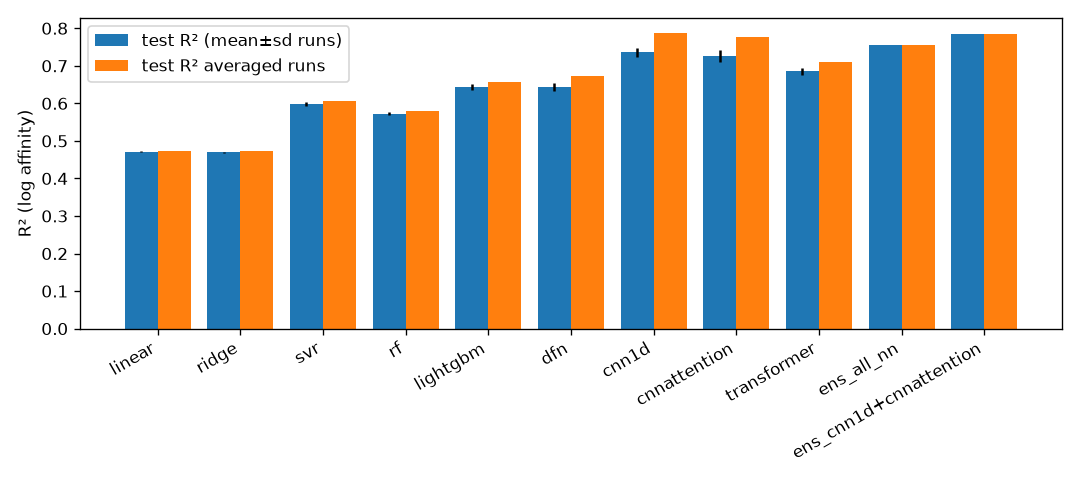
\includegraphics[width=.85\textwidth]{model_comparison.png}
\caption{Held-out test $R^2$ per model: mean$\pm$sd over runs, and the $R^2$ of the averaged prediction.}\label{fig:bar}\end{figure}

\begin{table}[H]\centering\small
\caption{Training dynamics of the neural networks (means over runs; MSE on standardised log affinity).}
\begin{tabular}{lcccc}\toprule
Model & Best epoch & Epochs run & Final train MSE & Best val MSE\\\midrule
DFN & 44.3 & 70.3 & 0.186 & 0.331 \\
CNN1D & 27.1 & 53.1 & 0.068 & 0.261 \\
CNNAttention & 21.6 & 47.6 & 0.055 & 0.266 \\
Transformer & 111.6 & 137.6 & 0.293 & 0.291 \\
\bottomrule\end{tabular}\label{tab:curves}\end{table}

\begin{figure}[H]\centering
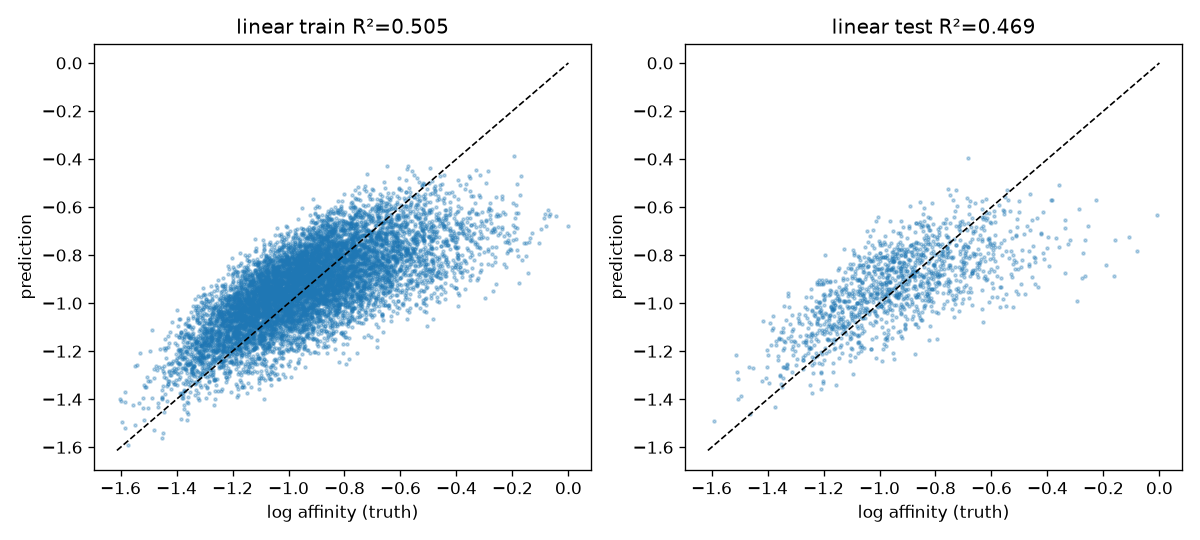
\includegraphics[width=.49\textwidth]{linear_truth_vs_pred.png}
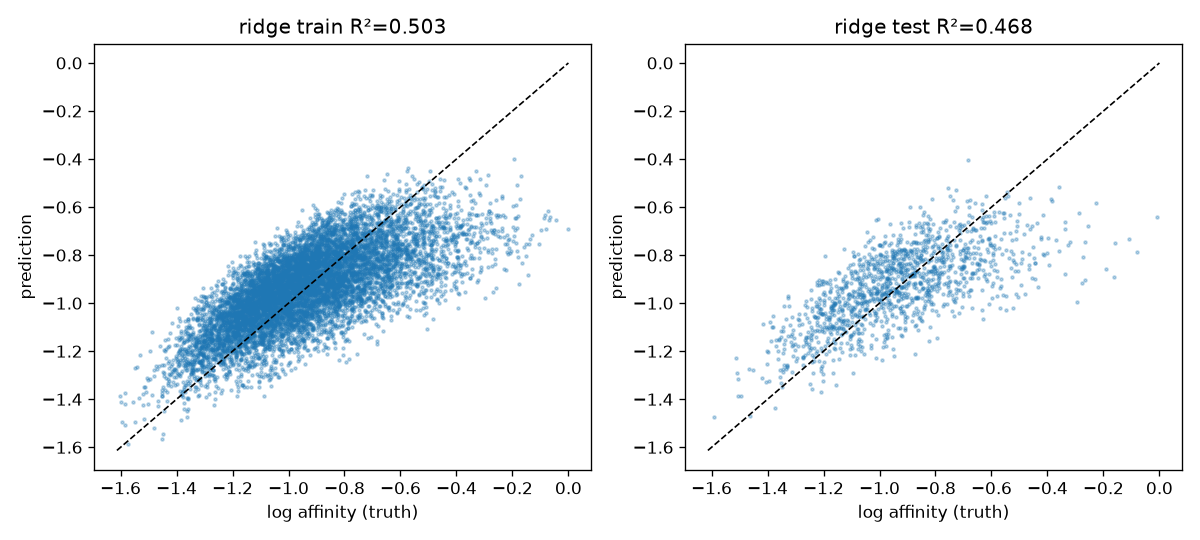
\includegraphics[width=.49\textwidth]{ridge_truth_vs_pred.png}
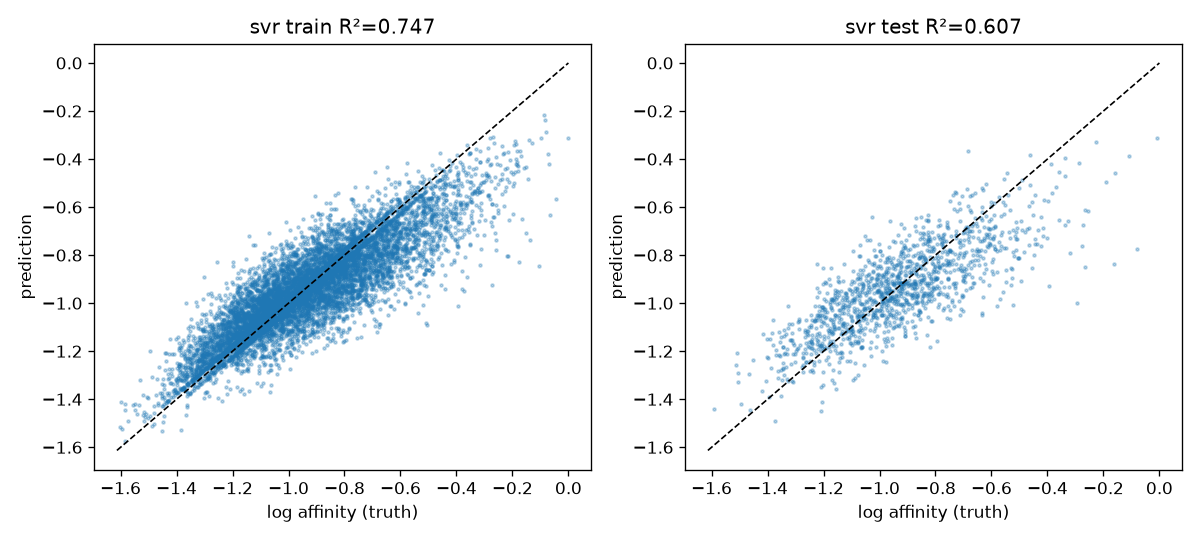
\includegraphics[width=.49\textwidth]{svr_truth_vs_pred.png}
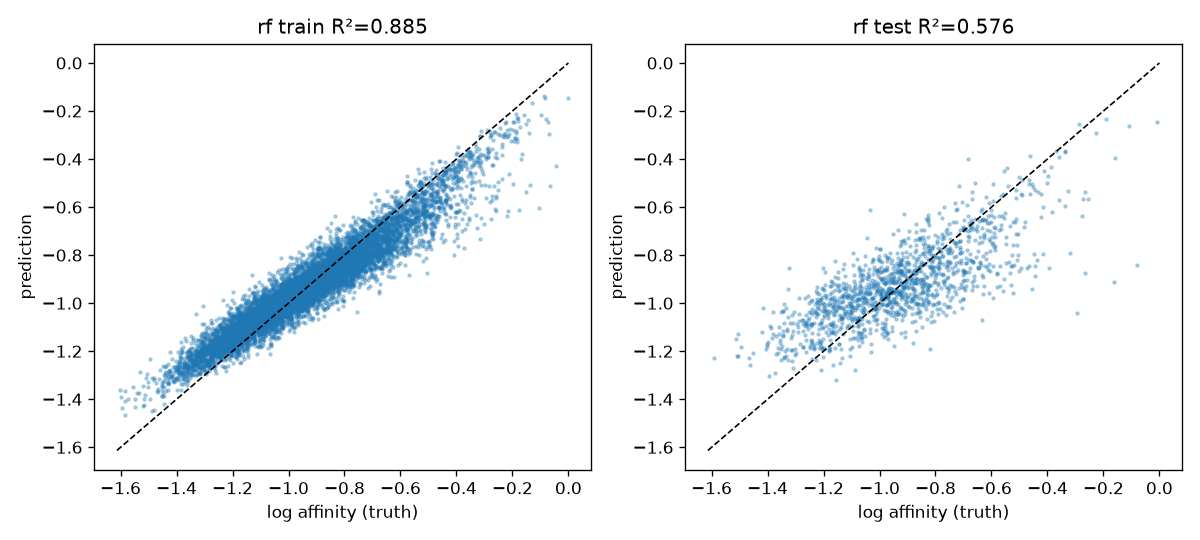
\includegraphics[width=.49\textwidth]{rf_truth_vs_pred.png}
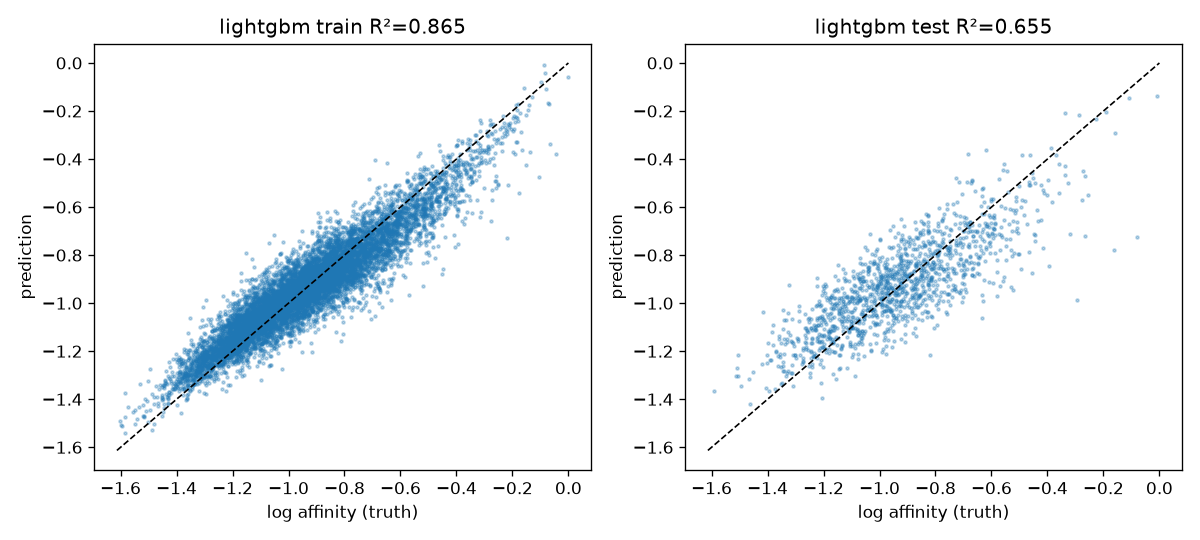
\includegraphics[width=.49\textwidth]{lightgbm_truth_vs_pred.png}
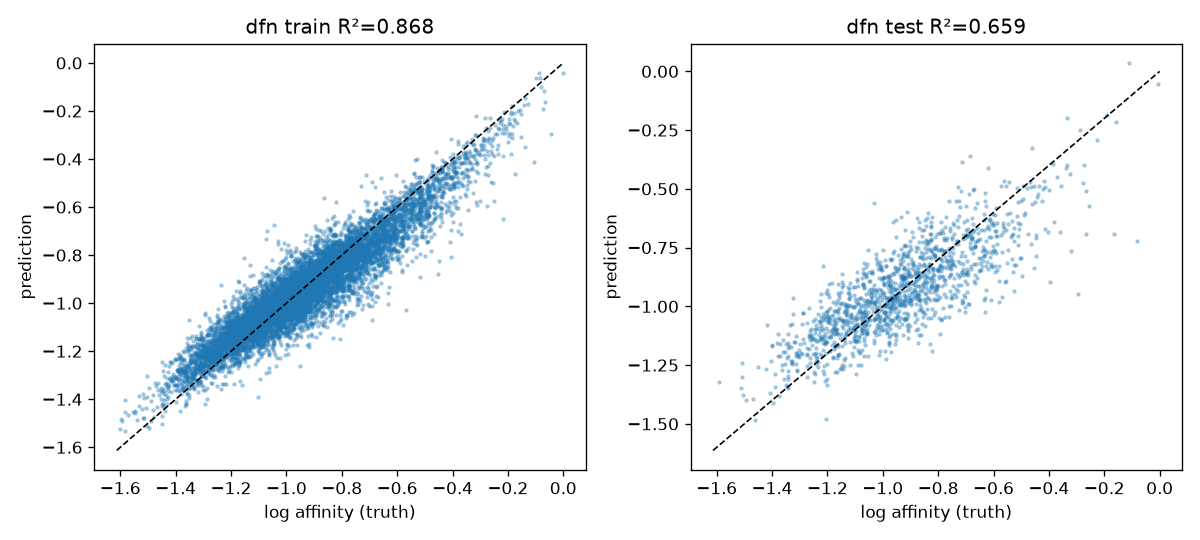
\includegraphics[width=.49\textwidth]{dfn_truth_vs_pred.png}
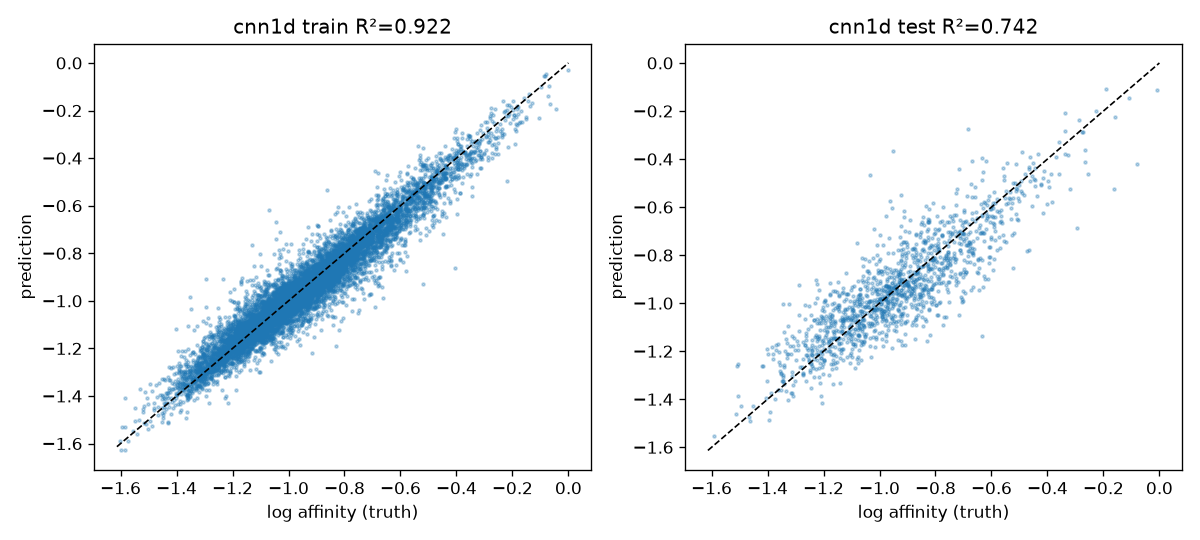
\includegraphics[width=.49\textwidth]{cnn1d_truth_vs_pred.png}
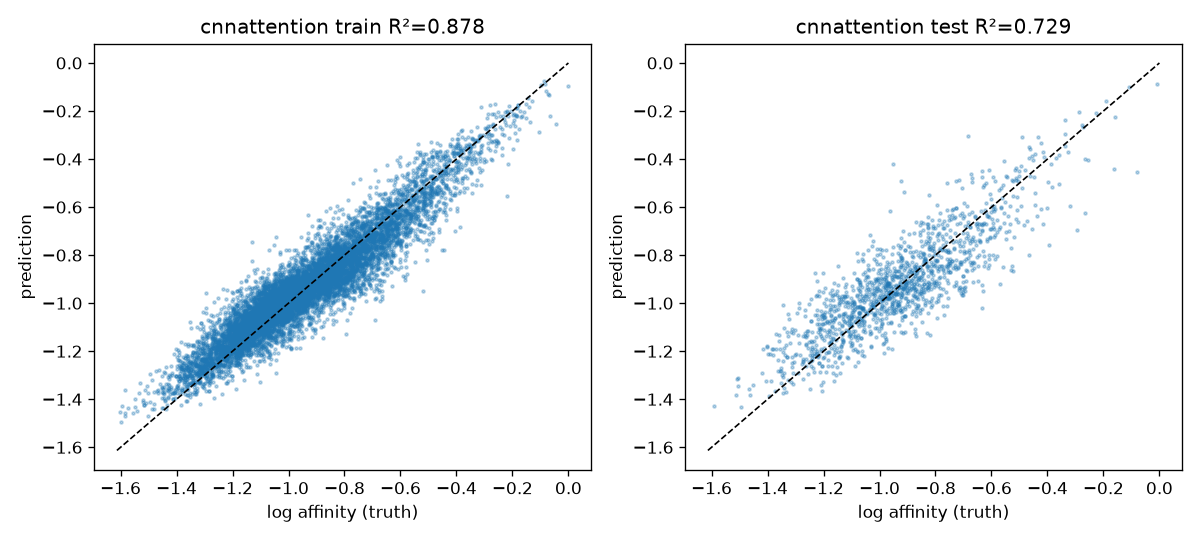
\includegraphics[width=.49\textwidth]{cnnattention_truth_vs_pred.png}
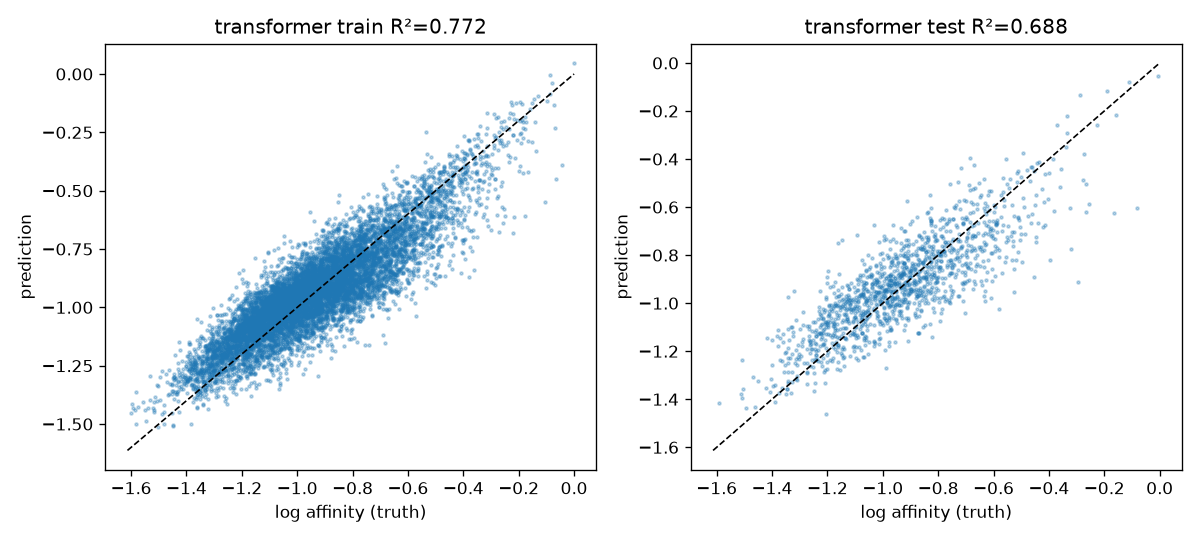
\includegraphics[width=.49\textwidth]{transformer_truth_vs_pred.png}
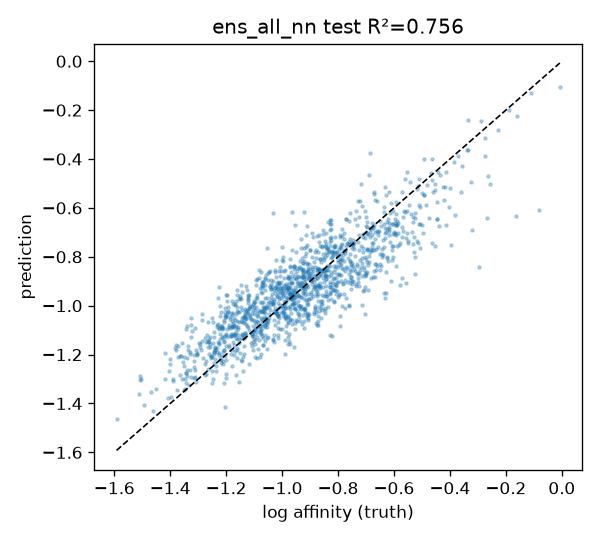
\includegraphics[width=.3\textwidth]{ens_all_nn_truth_vs_pred.png}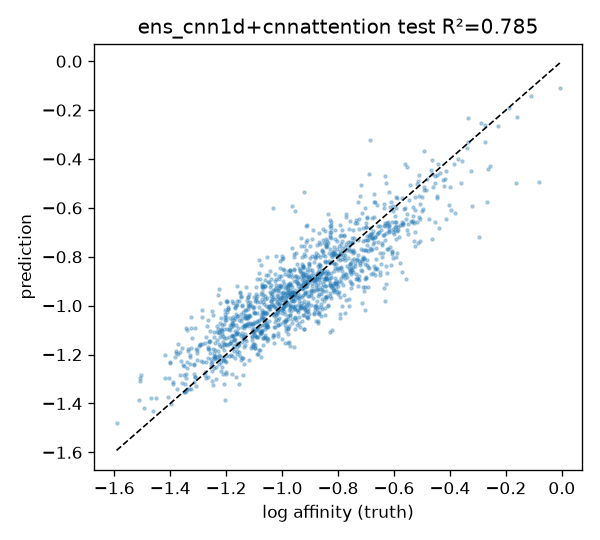
\includegraphics[width=.3\textwidth]{ens_cnn_attn_truth_vs_pred.png}
\caption{Ground truth vs.\ prediction (fold 0, seed 0) for each model on its training fold (left panel) and on the held-out test set (right panel), with $R^2$. The bottom row shows the two NN ensembles on the test set.}\label{fig:scatter}\end{figure}

\begin{figure}[H]\centering
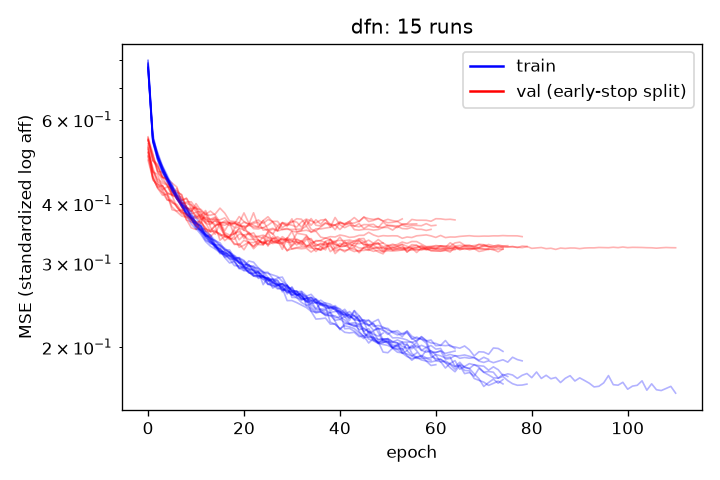
\includegraphics[width=.49\textwidth]{dfn_learning_curves.png}
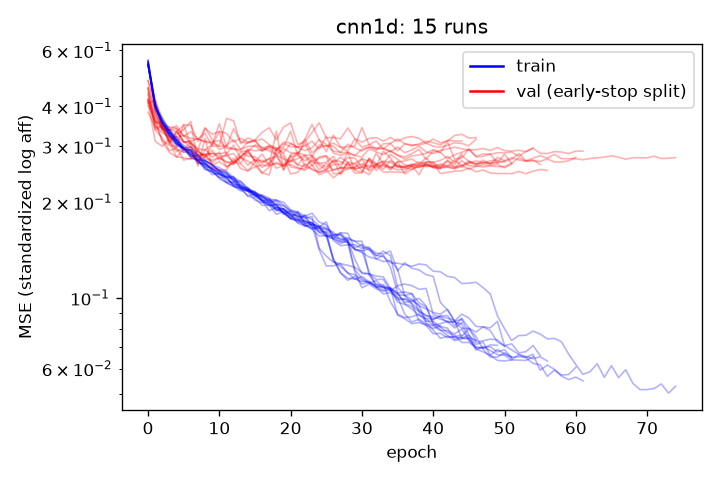
\includegraphics[width=.49\textwidth]{cnn1d_learning_curves.png}
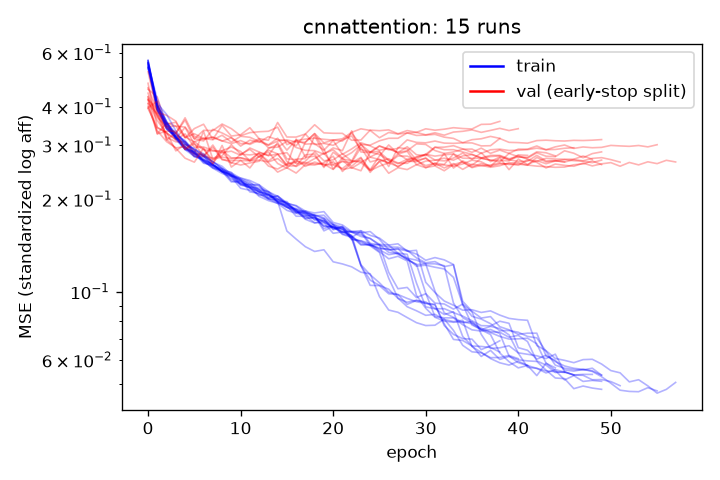
\includegraphics[width=.49\textwidth]{cnnattention_learning_curves.png}
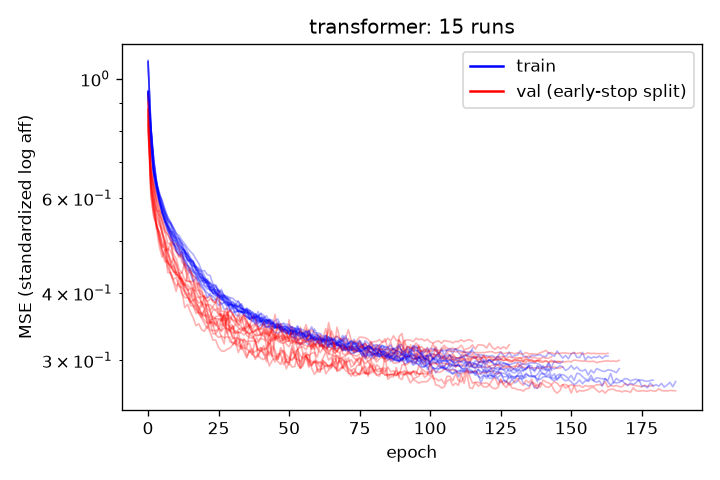
\includegraphics[width=.49\textwidth]{transformer_learning_curves.png}
\caption{Learning curves of all neural-network runs (blue: training loss, red: early-stopping validation loss).}\label{fig:curves}\end{figure}

\section{Discussion}
\paragraph{Strand asymmetry.} The two orientations of the same 10-mer correlate only $r\approx0.42$ in log affinity, and this does not improve when only high-count pairs are kept (0.425 at count $\geq$30). The asymmetry is therefore systematic, not counting noise. A likely cause is the orientation-dependent expected counts of the Markov background model, possibly combined with position or flank effects in the selection library. Averaging the two strands destroys this signal. Per-strand labels with reverse-complement-grouped CV improved CV $R^2$ by 0.15 (RF) and 0.17 (CNN1D) over merged labels.

\paragraph{Count threshold.} Counts below 10 add many labels whose relative SE is $\sqrt{2/n}$, i.e.\ $>45\%$. A threshold of 30 removes most low-affinity $k$-mers and biases predictions upwards on the shared evaluation rows. A threshold of 10 was the best trade-off. The log transform was marginally better than raw affinity.

\paragraph{Value of the shape features.} For the CNN, one-hot input alone matched one-hot plus shape (0.739 vs.\ 0.738). With 7 windows and 16 one-hot channels the network can learn the information in the shape lookup tables itself. For random forest, adding shape to one-hot helped (0.563 $\to$ 0.599). On their own, shape features are informative (CNN 0.692 without one-hot), and \texttt{fce} carried more signal than \texttt{avg}. Hexamer tables did not help: they are 96--99\% correlated with the central tetramer and enlarge the input.

\paragraph{Model comparison and overfitting.}
\begin{itemize}
\item Linear and ridge regression underfit (train $R^2$ 0.50, gap 0.03).
\item Random forest memorised the noisy labels (train 0.884, gap 0.31).
\item SVR and LightGBM generalised better (gaps 0.15 and 0.21).
\item The convolutional models were best. Their validation loss reached its minimum early (best epoch $\approx$22--27) while the training loss kept falling (final train MSE 0.05--0.07 vs.\ best validation MSE 0.26--0.27). This is overfitting, controlled by early stopping: validation and test $R^2$ agree closely (CNN1D 0.735 vs.\ 0.736), so there is no evidence of leakage.
\item The Transformer had the smallest gap (0.077) and nearly equal train and validation MSE (0.293 vs.\ 0.291). It trained longer (best epoch $\approx$112) and stayed underfit relative to the CNNs.
\item Averaging runs over folds and seeds helped the CNNs substantially (CNN1D 0.736 $\to$ 0.788). Adding the weaker DFN and Transformer to the ensemble lowered performance (0.756).
\end{itemize}

\paragraph{SELEX\_test.txt mismatch.} Only 8.4\% of the 5{,}511 10-mers in \texttt{SELEX\_test.txt} appear in \texttt{4.txt}. On the 462 shared $k$-mers its values are uncorrelated with the \texttt{4.txt} affinities (Pearson of logs $-0.03$, Spearman $-0.06$). Its scale is different (max 1.0, weights 1 or 10). It probably comes from another experiment or processing, so it was not used as a test set.

\paragraph{Limitations.} The ablation used a single seed and one-factor-at-a-time changes. We did not test de-duplication of shifted motif overlaps, or similarity-based grouping beyond reverse complements, so overlapping $k$-mers sharing a core motif can still occur on both sides of a split. Hyperparameters were not tuned per model. The only test data come from the same SELEX experiment.

\section{Conclusion}
The new MD shape tables are complete, internally consistent and differ measurably from the earlier tetramer tables. For Gata4 HT-SELEX the optimal preprocessing has five parts: log affinity, count $\geq$10, per-strand labels, tetramer avg+fce plus one-hot, and standardisation, all evaluated with reverse-complement-grouped CV. With this setup the CNN1D reaches a held-out test $R^2$ of 0.736 (0.788 when its runs are averaged) and is the best of the nine models compared, ahead of CNNAttention (0.725) and the Transformer (0.685). Shape features help tree models but are redundant for convolutional networks given one-hot input, and hexamer tables give no gain over tetramers. The main open issues are the strong strand asymmetry of the SELEX labels and the lack of an independent test set consistent with \texttt{4.txt}.

\begin{thebibliography}{9}
\bibitem{jolma2013} A.~Jolma \emph{et al.}, DNA-binding specificities of human transcription factors, \emph{Cell} 152, 327--339 (2013).
\bibitem{rohs2009} R.~Rohs \emph{et al.}, The role of DNA shape in protein--DNA recognition, \emph{Nature} 461, 1248--1253 (2009).
\end{thebibliography}
\end{document}
